\documentclass[t]{beamer}
\usepackage[utf8]{inputenc}  % to be able to type unicode text directly
%\usepackage[french]{babel}   % french typographical conventions
\usepackage{inconsolata}     % for a nicer (e.g. non-courier) tt family font
%\usepackage{amsthm,amsmath}  % fancier mathematics
\usepackage{array} % to fine-tune tabular spacing
\usepackage{bbm} % for blackboard 1

\usepackage{graphicx}        % to include images
%\usepackage{animate}         % to include animated images
\usepackage{soul}            % for colored strikethrough
%\usepackage{bbding}          % for Checkmark and XSolidBrush
\usepackage{hyperref,url}

\colorlet{darkgreen}{black!50!green}  % used for page numbers
\definecolor{term}{rgb}{.9,.9,.9}     % used for code insets

\setlength{\parindent}{0em}
\setlength{\parskip}{1em}


% coco's macros
\newcommand{\ds}{\displaystyle}
\def\R{\textbf{R}}
\def\C{\textbf{C}}
\def\K{\textbf{K}}
\def\N{\textbf{N}}
\def\F{\mathcal{F}}
\def\x{\textbf{x}}
\def\y{\mathbf{y}}
\def\u{\mathbf{u}}
\def\Z{\textbf{Z}}
\def\d{\mathrm{d}}
\DeclareMathOperator*{\argmin}{arg\,min}
\DeclareMathOperator*{\argmax}{arg\,max}
\newcommand{\reference}[1] {{\scriptsize \color{gray}  #1 }}
\newcommand{\referencep}[1] {{\tiny \color{gray}  #1 }}
\newcommand{\unit}[1] {{\tiny \color{gray}  #1 }}

% matrix groups and sets
\newcommand{\M}{\mathrm{M}}
\newcommand{\GL}{\mathrm{GL}}
\newcommand{\TS}{\mathrm{TS}}
\newcommand{\TI}{\mathrm{TI}}
\newcommand{\UU}{\mathrm{U}}
\newcommand{\OO}{\mathrm{O}}
\newcommand{\SO}{\mathrm{SO}}
\newcommand{\SU}{\mathrm{SU}}
\newcommand{\SL}{\mathrm{SL}}
\newcommand{\SSS}{\mathrm{S}}
\newcommand{\HH}{\mathrm{H}}

\newcommand{\parens}[1]{\left(#1\right)} % (x)
\newcommand{\pairing}[2]{\left\langle #1,#2\right\rangle} % <x,y>

% \abs{x}   ->    |x|
% \Abs{x}   ->   ||x||
% \ABS{x}   ->  |||x|||
\newcommand{\abs}[1]{\left|#1\right|}
\newcommand{\Abs}[1]{\left\|#1\right\|}
\newcommand{\ABS}[1]{{\left\vert\kern-0.25ex\left\vert\kern-0.25ex\left\vert #1 \right\vert\kern-0.25ex\right\vert\kern-0.25ex\right\vert}}

% disable spacing around verbatim
\usepackage{etoolbox}
\makeatletter\preto{\@verbatim}{\topsep=0pt \partopsep=0pt }\makeatother

% disable headings, set slide numbers in green
\mode<all>\setbeamertemplate{navigation symbols}{}
\defbeamertemplate*{footline}{pagecount}{\leavevmode\hfill\color{darkgreen}
   \insertframenumber{} / \inserttotalframenumber\hspace*{2ex}\vskip0pt}

%% select red color for strikethrough
\makeatletter
\newcommand\SoulColor{%
  \let\set@color\beamerorig@set@color
  \let\reset@color\beamerorig@reset@color}
\makeatother
\newcommand<>{\St}[1]{\only#2{\SoulColor\st{#1}}}
\setstcolor{red}

% make everything monospace
\renewcommand*\familydefault{\ttdefault}

\begin{document}

\begin{frame}[plain,fragile]
\LARGE
\begin{verbatim}



        ANALYSE NUMÉRIQUE 6/6

     Algèbre linéaire numérique :
         méthodes itératives



EML
30--11--2020
\end{verbatim}
\end{frame}

\begin{frame}[fragile]
PLAN\\
====

1. Aperçu des résultats principaux ({\bf 30min})

2. Travail par groupes ({\bf 90min})

3. Mise en commun ({\bf 60min})

\vfill
S.V.P.~: veuillez envoyer des retours (même anonymes) sur cette organisation à
\color{blue}\verb+enric.meinhardt@ens-paris-saclay.fr+
\vfill
\end{frame}

\begin{frame}
RAPPEL: {\bf LES} 4 PROBLÈMES DE L'ALGÈBRE LINÉAIRE NUMÉRIQUE\\
=======================================================

%Il y a seulement 4 problèmes en algèbre linéaire numérique.
Étant~$A\in\mathcal{M}_{m,n}(\K)$ de rang complet, %il faut
trouver~${\color{red}\x}\in\K^n$~:

{\color{blue} 1.}
\fbox{$A{\color{red}\x}=b,\quad A\in\mathcal{M}_{n,n}(\K)$}
%\pause
%Solution:~$x=A^{-1}b$.

%\pause
{\color{blue} 2.}
\fbox{$A{\color{red}\x}=b,\quad A\in\mathcal{M}_{m,n}(\K),\ m<n$}
%\pause
%Système sous-déterminé, espace affine de solutions.  Si~$A=[Q|S]$ alors
%$x=\left[Q^{-1}b-Q^{-1}S\mu\ |\ \mu\right]$ est solution~$\forall \mu\in\R^{n-m}$.

%\pause
{\color{blue} 3.}
\fbox{$A{\color{red}\x}=b,\quad A\in\mathcal{M}_{m,n}(\K),\ m>n$}
%\pause
%Système surdéterminé, pas de solution en général.
%\pause
%``Solution'' de moindres
%carrées: $\arg\min_x\left\|Ax-b\right\|^2=\left(A^TA\right)^{-1}A^Tb$.

``Solution'' pour
{\color{blue}1},
{\color{blue}2} et
{\color{blue}3}: $\x=A^\dagger b$\\
($A^\dagger=$ pseudo-inverse de Moore-Penrose)

\pause
{\color{blue} 4.}
\fbox{$A{\color{red}\x}=\lambda {\color{red}\x},\quad
A\in\mathcal{M}_{n,n}(\R)$}
\pause

Solutions pour~$\lambda\in\mathrm{sp}_{\C}(A)$, à calculer par approximations
itératives. {\color{blue}{\bf Bonus: } méthodes itératives pour~$A\x=b$.}

\end{frame}

\begin{frame}
APERÇU GÉNÉRAL\\
==============

\color{gray}
1. Algèbre et analyse matricielle\\
$\quad $ 1.1. Types de matrices\\
$\quad $ 1.2. Caractérisation du spectre\\
$\quad $ 1.3. Normes matricielles et conditionnement\\
$\quad $ 1.4. Décompositions: diagonalisation, polaire, SVD\\
$\quad $ 1.5. Pseudo-inverse de Moore-Penrose


2. Méthodes directes\\
$\quad $ 2.1. Complexité des opérations basiques\\
$\quad $ 2.2. Factorisations: LU, Cholesky, QR

\color{black}
3. Méthodes itératives\\
$\quad $ 3.1. Éléments propres\\
$\quad $ 3.2. Résolution d'un système (Jacobi, GS, grad, GC)

4. Modélisation\\
\end{frame}

% résultats du jour antérieur
\begin{frame}\small
RÉSULTATS DES DEUX JOURS ANTÉRIEURS\\
===================================

1. Théorème spectral:~$A=A^*\implies AV=V\Lambda$\\

%{\tiny\color{red}
%	 \(
%		\begin{pmatrix} a & b \\ b & c \end{pmatrix}
%		\begin{pmatrix} b & a-\lambda \\ \lambda-a & b \end{pmatrix}
%		=
%		\begin{pmatrix} b & a-\lambda \\ \lambda-a & b \end{pmatrix}
%		\begin{pmatrix} \lambda & 0 \\ 0 & \mu \end{pmatrix}
%	\),
%	$\ $ avec~$ \lambda,\mu =\displaystyle
%	\tfrac12\left({a+c\pm\sqrt{(a-c)^2+4b^2}}\right) $
%}

2. Caractérisations de~$\mathrm{sp}(A)$, %: alg., géo., optim.,
$\mathrm{sp}(A)\subseteq\mathcal{G}(A),\ldots$\\

3. Pseudo-inverse: $Ax=b$ est ``résolu'' par~$x=A^\dagger b$ %, avec~$A^+$
%unique satisfaisant~{\color{blue}$AA^\dagger A=A$, $\ A^\dagger AA^\dagger=A^\dagger$, $\ (AA^\dagger)^*=AA^\dagger$,
%	$\ (A^\dagger A)^*=A^\dagger A$.
%	}

4. Décompositions et factorisations:\\
$\ $4.0. Diagonalisation: $A=S^{-1} D S$\\
$\ $4.1. Polaire: $\GL_n(\C)=\HH_n^{++}(\C)\times\UU_n(\C)$\\
$\ $4.2. SVD: $\M_{p,q}(\C)\approx \UU_p(\C)\times \mathrm{diag}^+_{p,q}(\R) \times \UU_q(\C)$\\
$\ $4.3. Gauss/LU: $A=LU\in\TI^1_n(\K)\times\TS_n(\K)$\\
$\ $4.4. Cholesky: $\HH_n^{++}(\C)\ni A=BB^*\in\TI_n^{++}(\C)\times\TS_n^{++}(\C)$\\
$\ $4.5. QR: $\GL_n(\C)=\UU_n(\C)\times\TS_n^{++}(\C)$

5. Normes matricielles:\\
$\ $5.1. Normes induites~$\displaystyle\ABS{A}_\alpha=\inf_{\|x\|_{\alpha}=1}\|Ax\|_{\alpha}$, $\ \ABS{A}_2=\sqrt{\rho(AA^*)}$\\
$\ $5.2. Th. Householder:~$\rho(A)=\displaystyle\inf_{\ABS{\phantom{\cdot}}}\ABS{A}$\\
$\ $5.3. Convergences:~$\color{blue}(I-A)^{-1}=I+A+A^2+\cdots$ si~$\ABS{A}<1$,\\
$\qquad\qquad\displaystyle\color{blue}\mathrm{\rho}(A)
=\lim_{k\to\infty}\ABS{A^k}^{1/k}$,
etc

\end{frame}

% interlude: résolution d'équations non-linéaires
\begin{frame}
INTÉRLUDE: RÉSOLUTION D'ÉQUATIONS NON-LINÉAIRES\\
===============================================

{\bf Problème 1D:}\\
Étant donnée~$f:\R\to\R$, trouver~$x\in\R$ tel que~$f(x)=0$


Et plus en général:

{\bf Problème nD:}\\
Étant donnée~$f:\R^n\to\R^n$, trouver~$\x\in\R^n$ tel que~$f(\x)=0$

\end{frame}

% méthode de la subdivision
\begin{frame}
MÉTHODE DE LA SUBDIVISION\\
=========================

Pour~$f:[a,b]\to\R$ continue avec~$f(a)f(b)<0$.

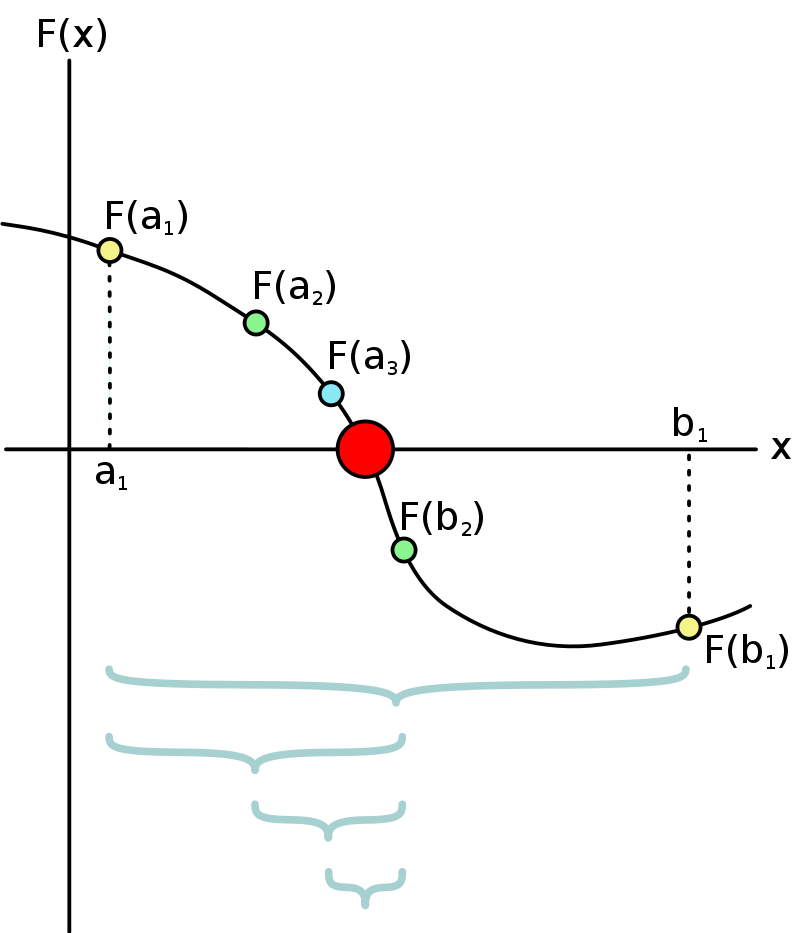
\includegraphics[width=0.4\linewidth]{f/bisection.png}

\pause
{\bf Analyse:} L'erreur absolu se divise par deux à chaque itération
(convergence linéaire): $\abs{x_n-x}\le\abs{b-a}/2^n$.
\end{frame}

% méthode de newton
\begin{frame}
MÉTHODE DE NEWTON\\
=================

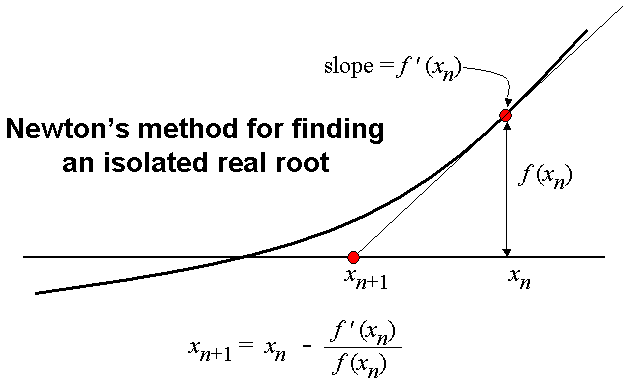
\includegraphics[width=0.7\linewidth]{f/newton.png}

{\bf Méthode:} À partir d'un~$x_0$ quelconque, on fait des
itérations~$x_{n+1}:=x_n-f(x_n)/f'(x_n)$.

{\bf Analyse:} En conditions favorables, on a convergence quadratique
$\abs{x_{n+1}-x}<C\abs{x_n-x}^2$.
\end{frame}

% méthode de newton
\begin{frame}
ANALYSE DE LA MÉTHODE DE NEWTON {\color{red}\bf(Exercice N.)}\\
===========================================

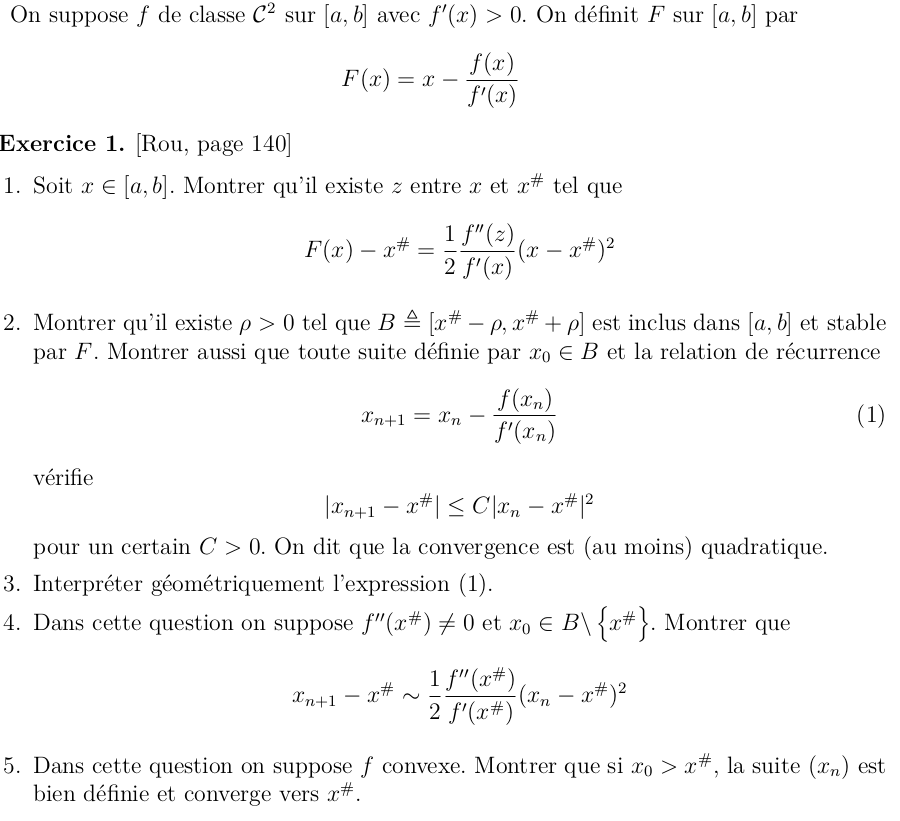
\includegraphics[height=0.8\textheight]{f/exernewton.png}
\end{frame}

% newton pour polynômes
\begin{frame}
MÉTHODE DE NEWTON POUR POLYNÔMES {\color{red}\bf(Exercice N'.)}\\
===========================================

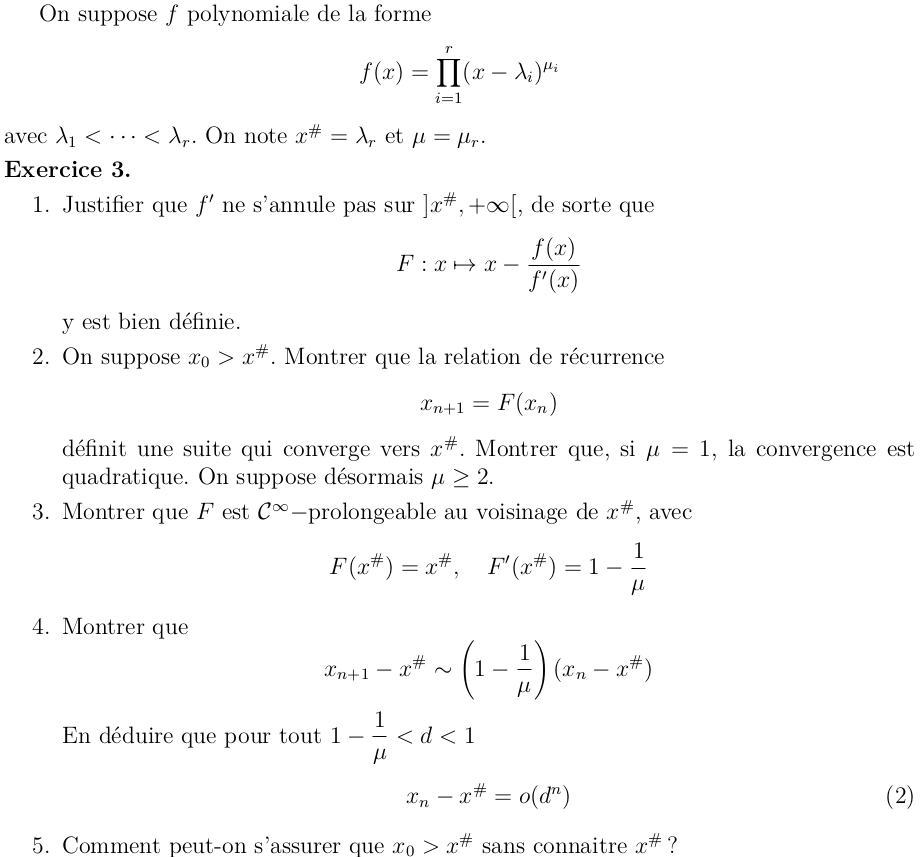
\includegraphics[height=0.8\textheight]{f/exernewton2.png}
\end{frame}

% newton counterexample sigmoid
\begin{frame}
NON-CONVERGENCE DE LA MÉTHODE DE NEWTON\\
=======================================

Les racines de~$f(x)$ sont des attracteurs pour la méthode de Newton.  En
dehors de ses puits d'attraction, les itérés peuvent devenir périodiques, ou
aller vers~$\infty$

\pause
{\bf Exemples?}

\pause
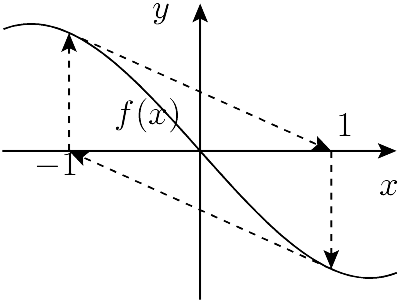
\includegraphics[height=0.5\textheight]{f/newtoncycle.png}
\end{frame}

% newton fractal
\begin{frame}
MÉTHODE DE NEWTON EN nD\\
=======================

Soit~$F:\R^n\to\R^n$, par analogie avec le cas de dimension 1
\[
	x_{n+1}:=x_n-f(x_n)/f'(x_n)
\]
on définit les itérés e pour~$F$:
\[
	\x_{n+1}:=\x_n-\left(DF(\x_n)\right)^{-1} F(\x_n)
\]
c'est la méthode de Newton en dimension~$n$, avec des propriétés très
similaires.
\end{frame}

% newton fractal
\begin{frame}
MÉTHODE DE NEWTON POUR POLYNÔMES $P:\C\to\C$\\
=========================================

Soit~$f:\C\to\C$ définie par
\[f(z)=z^3-1\color{gray}=(z-1)(z-\rho)(z-\overline\rho)\]
Le plan~$\C$ est divisé en 3 parties associées à chaque attracteur.
Quelle est la forme de ces parties?

\pause
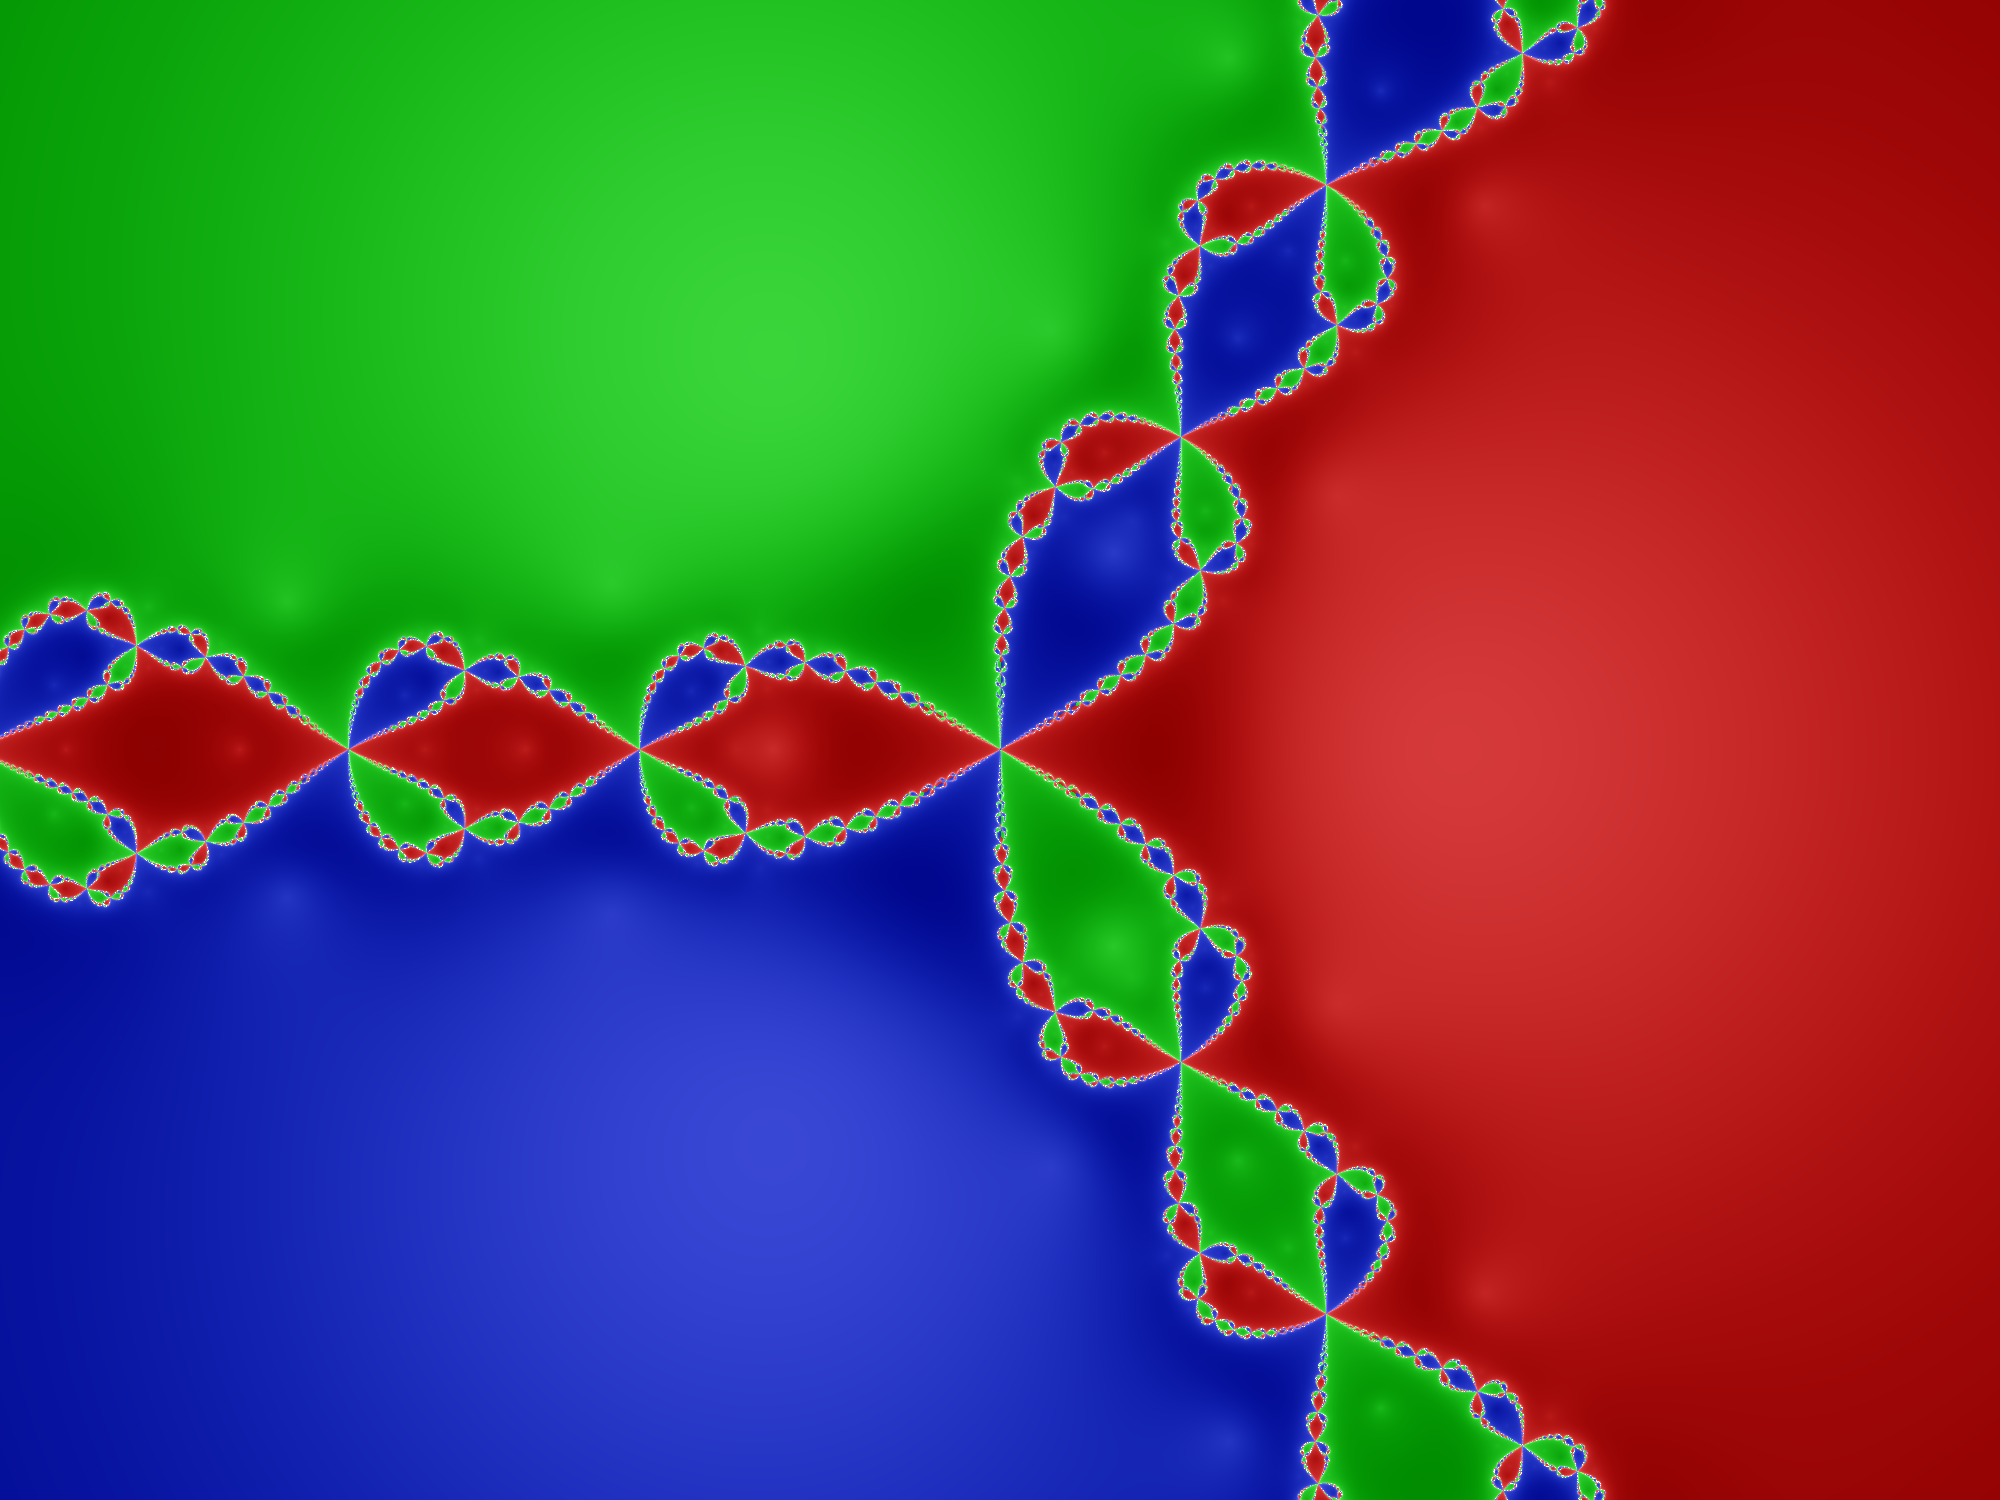
\includegraphics[height=0.5\textheight]{f/juliacube.png}
\end{frame}

% super-slide méthode de newton
\begin{frame}
LA MÉTHODE DE NEWTON: OPTIMISATION VS RÉSOLUTION\\
================================================

{\bf Résolution.}  Pour~$F:\R^n\to\R^n$, trouver~$\x$ tel que $F(\x)=0$~:
\[
	\x_{n+1}:=\x_n-\left(DF(\x_n)\right)^{-1} F(\x_n)
\]

{\bf Optimisation.}
Pour~$f:\R^n\to\R$, trouver~$\x=\argmin f(\x)$~:
\[
	\x_{n+1}:=\x_n-\left(D^2f(\x_n)\right)^{-1} Df(\x_n)
\]

\pause
{\bf Lien~:} minimiser~$f(\x)$ équivaut à résoudre~$Df(\x)=0$.
\end{frame}


% polynômes vs matrices
\begin{frame}
POLYNÔMES ET MATRICES\\
=====================

Soit~$\displaystyle P(X)=X^n+\sum_{k=0}^{n-1}c_k X^k$ un polynôme unitaire
de~$\C_n[X]$.  La matrice~{\color{blue}compagnon} de~$P$~:

\[
	\mathcal{C}(P)=
	\left(\begin{array}{cccc}
			0 & \dots & 0 & -c_0 \\
			1& \ddots &\vdots  & \vdots \\
			& \ddots & 0 & \vdots \\
			&  & 1 & -c_{{n-1}}
	\end{array}\right) \in\M_n(\K)
\]

a pour valeurs propres les racines de~$P$.

\pause
{\bf Observation:} Ainsi, toute méthode générale de calcul d'éléments propres
d'une matrice pour~$n>4$ est forcément itératif (il donne une suite
d'approximations successives des éléments propres).
\end{frame}

%% méthode de newton pour les polynômes [EX]
%\begin{frame}
%MÉTHODE DE NEWTON POUR POLYNÔMES: ANALYSE\\
%=========================================
%\end{frame}






% méthodes itératives, considérations générales (points fixes)
\begin{frame}
MÉTHODES ITÉRATIVES POUR PROBLÈMES LINÉAIRES\\
============================================

{\bf Idée:} transformer le problème ($Ax=b$ ou~$Ax=\lambda x$)
en~$\color{blue}F(y)=y$ et appliquer un théorème de point fixe qui garantira la
convergence des itérés~$y_{n+1}:=F(y_n)$% vers la solution.

{\bf Th. (point fixe de Banach).}  Soit~$k<1$ et~$F:V\to V$~$k$-Lipschitzienne
sur un e.m. complet~$V$.  Alors il existe un unique~$x\in V$ tel que~$F(x)=x$, et~$\forall a\in V$ on a~$\displaystyle\lim_{n\to\infty}F^n(a)=x$.

{\bf Th. (point fixe de Browder-Kirk).}
Soit~$C\subseteq E$ une partie convexe, bornée et fermée d'un espace de
Banach~$E$, et~$F:C\to C$ non-expansive ($\Abs{F(x)-F(y)}\le\Abs{x-y}$).
Alors~$F$ a un point fixe (pas forcément unique).

\end{frame}

% méthodes itératives, trois types ici ensuite
\begin{frame}
TROIS TYPES DE MÉTHODES ITÉRATIVES\\
==================================

Par ordre croissant de difficulté:

1. Étant donnée~$A\in\M_n(\K)$, construire une suite~$(\lambda^k,\x^k)$ qui
s'approche à une solution de~$A\x=\lambda\x$.\\
\uncover<2>{{\color{blue}Méthodes de la puissance, puissance inverse.}}

2. Étant donnée un système linéaire inversible~$A\x=b$, construire une
suite~$\x^k$ qui s'approche à la solution
\uncover<2>{{\color{blue}Jacobi, Gauss-Seidel, S.O.R., Gradient pas fixe,
Gradient pas optimal, Gradients conjugués.}}

3. Étant donnée une matrice diagonalisable~$A$, approcher l'ensemble entier de
ses éléments propres.\\
\uncover<2>{{\color{blue}Algorithme QR (basé sur la décomposition QR).}}
\end{frame}


% méthode de la puissance
\begin{frame}
MÉTHODE DE LA PUISSANCE\\
=======================

{\bf Principe.}
On construit une suite $({\color{blue}x^k})$ par récurrence~:
\[
	{\color{blue}x^0} \in \K^n\ \textrm{quelconque}, \qquad {\color{blue}x^{k+1}}
	:= \frac{A{\color{blue}x^k}}{{\Abs{A{\color{blue}x^k}}}}
\]

{\bf Proposition.}
Soit~$A$ diagonalisable à valeurs propres réelles
$|\lambda_1|\le\cdots\le|\lambda_{n-1}|<|\lambda_n|$ et~$\color{red}\tau=|\lambda_{n-1}|/|\lambda_n|<1$.
Alors~:\\
1. ${\color{blue}x^k}$ converge ${\color{red}\tau}$-linéairement vers un vec. propre de~$A$\\
2. $\Abs{A {\color{blue}x^k}}=\lambda_n+\mathcal{O}({\color{red}\tau}^k)$\\
3. $\Abs{A {\color{blue}x^k}}=\lambda_n+\mathcal{O}({\color{red}\tau}^{2k})$
pour~$A$ symétrique, hermitienne


\vfill
\color{red}
{\bf Exercice 36.}\\ Démontrez cette proposition (cf. notes pp.23--24).

\end{frame}

% notion de taux de convergence [EX]
%\begin{frame}
%MÉTHODE DE LA PUISSANCE: TAUX DE CONVERGENCE\\
%============================================
%\end{frame}

% méthode de la puissance inverse [EX]
\begin{frame}
MÉTHODE DE LA PUISSANCE INVERSE\\
===============================

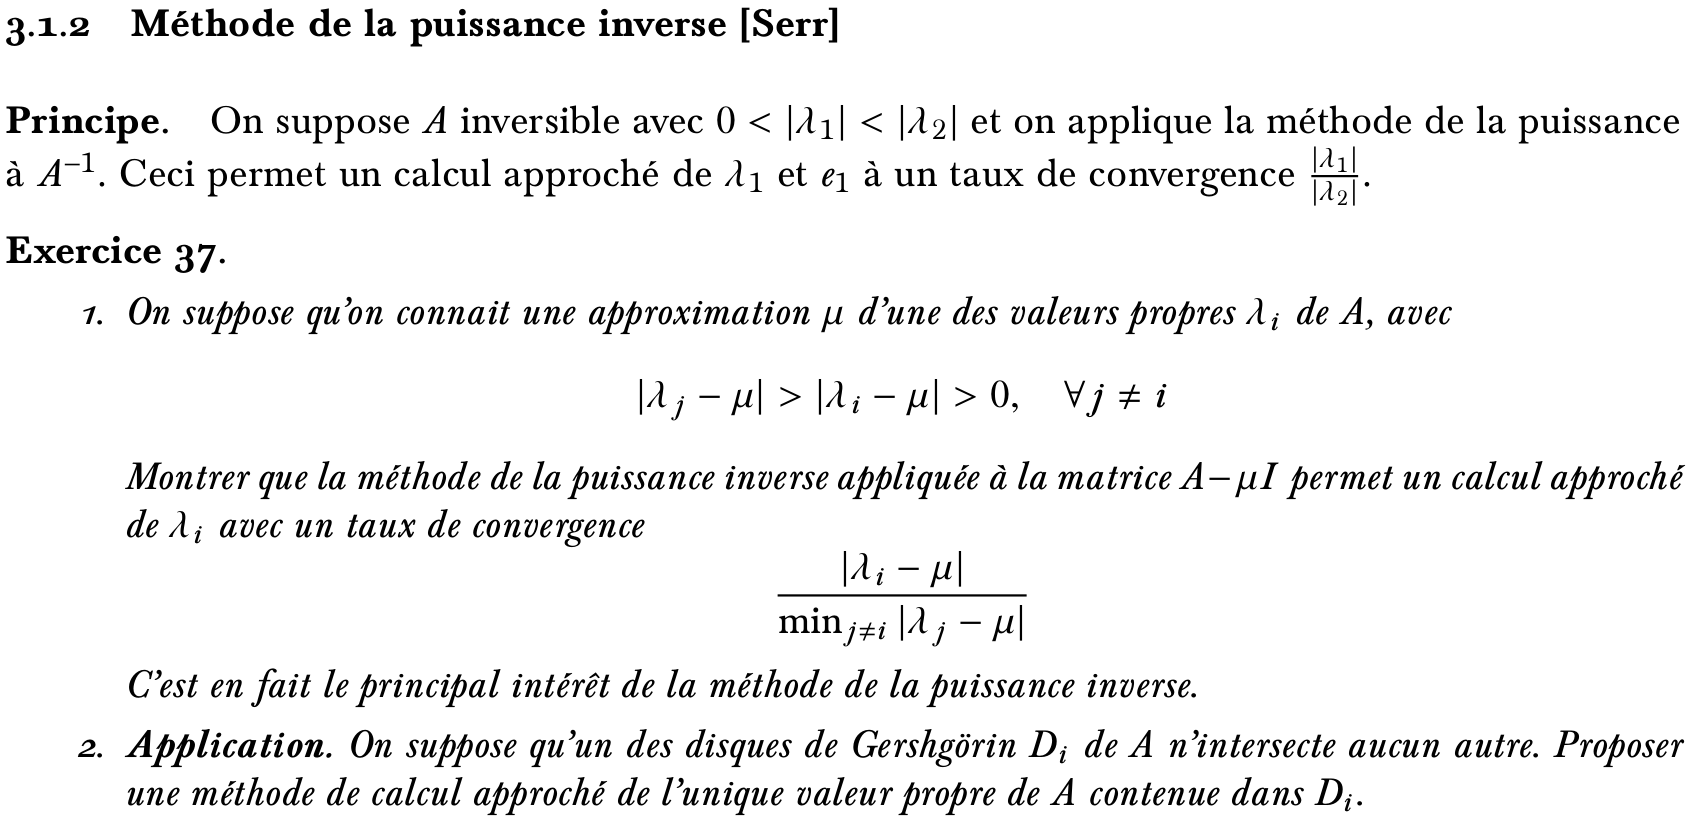
\includegraphics[width=\linewidth]{f/puissanceinverse.png}

\vfill
\color{red}{\bf Exercice 37.}
\end{frame}

% algorithme QR
\begin{frame}
ALGORITHME QR\\
=============

L'algorithme~$QR$ utilise des décompositions QR successives pur
{\color{blue}approcher l'ensemble de tous les éléments propres}.

{\bf Algorithme}.  Étant donnée~$A\in\GL_n(\R)$, on construit la suite de
matrices~$A_k$ par récurrence:
\[
	A_1=A
	\qquad\qquad
	A_{k+1}:=R_kQ_k
\]
où~$(Q_k,R_k)$ est la factorisation~$QR$ de~$A_k$.

\pause
{\bf Th.9 (convergence de l'algorithme QR).}
Soit~$A$ diagonalisable~$A=Y^{-1}DY$
avec~$D=\mathrm{diag}(\lambda_1,\ldots,\lambda_n)$
et~$|\lambda_1|>\cdots>|\lambda_n|>0$, telle que~$Y$ admet une
décomposition~$LU$.  Alors la partie triangulaire inférieure de~$A_k$
converge vers~$D$.
\color{red}\bf(Exercice 44.)
\end{frame}



% méthodes itératives de résolution (forme générale)
\begin{frame}\small
MÉTHODE ITÉRATIVES DE RÉSOLUTION : CADRE GÉNÉRAL\\
================================================

{\bf Idée:}
Pour résoudre~$Ax=b$ on décompose~$A=M-N$
%Soit~$A\in\GL_n(\K)$ et~$b\in\K^n$, on veut trouver~$x\in\K^n$ tel
%que~$Ax=b$.
%Le principe de base est de décomposer $A$ en
%\[
%A = M - N
%\]
avec $M$ inversible, de sorte que
\[
Ax = b \quad \Leftrightarrow \quad Mx = Nx + b \quad \Leftrightarrow \quad x = M^{-1}(Nx+b)
\]
La méthode %itérative associée à la décomposition $A = M-N$
consiste alors à
choisir $x^0 \in \K^{n}$ et à calculer les itérés $x^k$ solution de
\[
Mx^{k+1} = (Nx^k + b)
\qquad\qquad
%\color{gray}
%x^{k+1} = M^{-1}(Nx^k + b)
\]

{\bf Observation.}
Ceci n'a d'intérêt que si $M$ facilite le travail (e.g. $M$ diagonale ou
triangulaire).
La pertinence de la décomposition se lit sur le rayon spectral de $M^{-1}N$.

{\bf Proposition.}
La suite $(x^k)$ converge vers $x=A^{-1}b$ quelque soit $x^0$ si
et seulement si $\rho(M^{-1}N) < 1$.
%On dit alors que la méthode est convergente.
{\bf\color{red}(Exercice 38.)}

%\begin{exercice}
%Prouver la Proposition \ref{prop:methodes_iteratives}. Montrer que la
%convergence est au moins linéaire et donner le taux de convergence.
%\end{exercice}
%
%
%{\bf Algorithmique.}
%En pratique on ne connait pas la solution $x$ (on en cherche une approximation !) donc on ne sait pas quel terme $x^k$ est satisfaisant. Un critère souvent utilisé est de s'arrêter lorsque
%\[
%\Abs{Ax^k-b} \leq \epsilon
%\] 
%où $\epsilon$ est un seuil défini à l'avance. On note $K$ le nombre d'itérations effectuées avant l'arrêt. En pratique, la complexité des méthodes itératives est en $Kn^2$. Elles sont donc intéressantes si $K \ll n$.

{\bf Remarque.}
C'est la méthode de point fixe pour la fonction $x \mapsto (M^{-1}N x +b)$. L'inégalité $\rho(M^{-1}N) < 1$ équivaut au fait que la fonction est contractante.

\end{frame}

% méthode de Jacobi
\begin{frame}
MÉTHODE DE JACOBI\\
=================

On prend~$M$ la diagonale de~$A$.  Par exemple
\[
A = \left(\begin{array}{ccc}
1 & 2 & 0 \\
2 & 13 & 2 \\
 1 & 1 & 2
\end{array}\right)
, \quad M = \left(\begin{array}{ccc}
1 & 0 & 0 \\
0 & 13 & 0 \\
 0 & 0 & 2
\end{array}\right)
, \quad N = \left(\begin{array}{ccc}
0 & -2 & 0 \\
-2 & 0 & -2 \\
-1 & -1 & 0
\end{array}\right)
\]

{\color{red}\bf Exercice 39.}
On suppose que $A$ est à diagonale strictement dominante. Montrer que la
méthode de Jacobi pour~$A$ est convergente.

\vfill
\color{blue}
\fbox{$Mx^{k+1}=Nx^k+b$}
\end{frame}

% méthode de Gauss-Seide [EX]
\begin{frame}
MÉTHODE DE GAUSS-SEIDEL\\
=======================

On prend $M$ la partie triangulaire inférieure de $A$, par exemple
\[
A = \left(\begin{array}{ccc}
1 & 2 & 0 \\
2 & 13 & 2 \\
1 & 1 & 2
\end{array}\right)
, \quad M = \left(\begin{array}{ccc}
1 & 0 & 0 \\
2 & 13 & 0 \\
1 & 1 & 2
\end{array}\right)
, \quad N = \left(\begin{array}{ccc}
0 & -2 & 0 \\
0 & 0 & -2 \\
0 & 0 & 0
\end{array}\right)
\]

{\bf Proposition.}
Si $A \in\HH^{++}_n(\C)  $ alors la méthode de Gauss-Seidel est convergente.

{\bf\color{red} Exercice 40.} Démontrez la proposition.  Indications~:\\
1. Démontrez que~$M^*+N$ est diagonale et déf. positive\\
2. Démontrez que~$\Abs{M^{-1}N}_A^2<\Abs{x}^2_A$ (avec~$\Abs{x}_A=\sqrt{x^TAx}\ $)\\
3. Conclure

{\bf Remarque.} De manière générale, la méthode est convergente
quand~$A\in\HH^{++}_n(\C)$
et~$M^*+N\in\HH^{++}_n(\C)$.
\end{frame}

% méthode de Gauss-Seidel avec sur-relaxation
\begin{frame}
MÉTHODE DE SUR-RELAXATION\\
=========================

Un raffinement de la méthode de Gauss-Seidel consiste à pondérer la diagonale
de $A$ dans $M$ par un facteur $\frac{1}{\omega}$. Par exemple pour $\omega =
\frac{1}{3}$
\[
A = \left(\begin{array}{ccc}
1 & 2 & 0 \\
2 & 13 & 2 \\
1 & 1 & 2
\end{array}\right)
, \quad M = \left(\begin{array}{ccc}
3 & 0 & 0 \\
2 & 39 & 0 \\
1 & 1 & 6
\end{array}\right)
, \quad N = \left(\begin{array}{ccc}
2 & -2 & 0 \\
0 & 26 & -2 \\
0 & 0 & 4
\end{array}\right)
\]
C'est la \emph{méthode de relaxation} [Serr,~chap.~9]
convergente si et seulement si $|\omega-1| < 1$. L'idée est de choisir
judicieusement $\omega$ pour rendre $\rho(M^{-1}N)$ le plus petit possible,
accélérant ainsi la convergence.
\end{frame}

% exemples sur le laplacien 1D
\begin{frame}
EXEMPLES POUR LE LAPLACIEN DISCRET
==================================

L'opérateur de dérivé seconde $\color{blue}(u_i)'':=u_{i-1}-2u_i+u_{i+1}$
correspond à une matrice~$L$ symétrique négative.

L'équation ``de poisson discrète'' $-Lu=f$ peut se résoudre ainsi par Jacobi,
Gauss-Seidel, SOR.  Ces méthodes correspondent à l'évolution de l'équation de
la chaleur avec source~$u_t=\Delta u +f$, pour {\color{red}différents choix}
d'implémentation de la dérivée temporelle:

\[
	\frac{u^{n+1}_i-u^n_i}{\tau}=(u^n_i)''-f_i
\]

%{\bf G.S.} $x^{u+1} := 
{\color{red}{\bf Exercice P. } Précisez et vérifiez ces choix.}\\
\color{gray}Indication: $\tau=1/4$ pour Jacobi et GS,~$\tau=1/2-\omega$ pour~$SOR$

\end{frame}

% résolution via optimisation
\begin{frame}
RÉSOLUTION PAR OPTIMISATION\\
===========================

{\bf Idée:}  Si~$A\in\SSS^{++}_n(\R)$, alors résoudre
\[
	Ax=b
\]
est équivalent à minimiser cette fonction~$F:\R^n\to\R$
\[
	F(x)=\frac12 x^TAx-b^Tx
\]

\pause{\color{darkgreen}{\bf Question:} Est-il envisageable d'utiliser la
méthode de Newton ici?
}
\pause
\[
	DF(x) = Ax-b
\]
\[
	D^2F(x) = A
\]

\end{frame}

% descente de gradient pas fixe [EX]
\begin{frame}
DESCENTE DE GRADIENT\\
====================

Dans cette méthode $M = \frac{1}{\alpha} I$, où $\alpha \in \R^*$ est un
paramètre de réglage. Par exemple pour $\alpha = 0.1$
{\tiny
\begin{displaymath}
A = \left(\begin{array}{ccc}
1 & 2 & 0 \\
2 & 13 & 2 \\
 1 & 1 & 2
\end{array}\right)
, \quad M = \left(\begin{array}{ccc}
10 & 0 & 0 \\
0 & 10 & 0 \\
 0 & 0 & 10
\end{array}\right)
, \quad N = \left(\begin{array}{ccc}
9 & -2 & 0 \\
-2 & -3 & -2 \\
-1 & -1 & 8
\end{array}\right)
\end{displaymath}
}

{\bf\color{red}Exercice 41.}
Soit $A$ de valeurs propres $0 < \lambda_1 < \dots <\lambda_n$:\\
1. Montrez que la suite des itérés est
\begin{displaymath}
x^{k+1} = x^{k} - \alpha (Ax^k -b)
\end{displaymath}
et justifier le nom de la méthode.\\
2. Montrez convergence sii  $0 < \alpha < \frac{2}{\rho(A)}$.\\
3. Montrez que \( \alpha = \frac{2}{\lambda_1 + \lambda_n} \)
minimise $\rho(M^{-1}N)$ qui vaut alors
\begin{displaymath}
\rho(M^{-1}N) = \frac{\lambda_n - \lambda_1}{\lambda_n + \lambda_1}
\end{displaymath}
\end{frame}

% descente de gradient pas optimal [EX]
\begin{frame}
DESCENTE DE GRADIENT À PAS OPTIMAL\\
==================================

\vfill\color{red}\bf Exercice 42.

\vfill

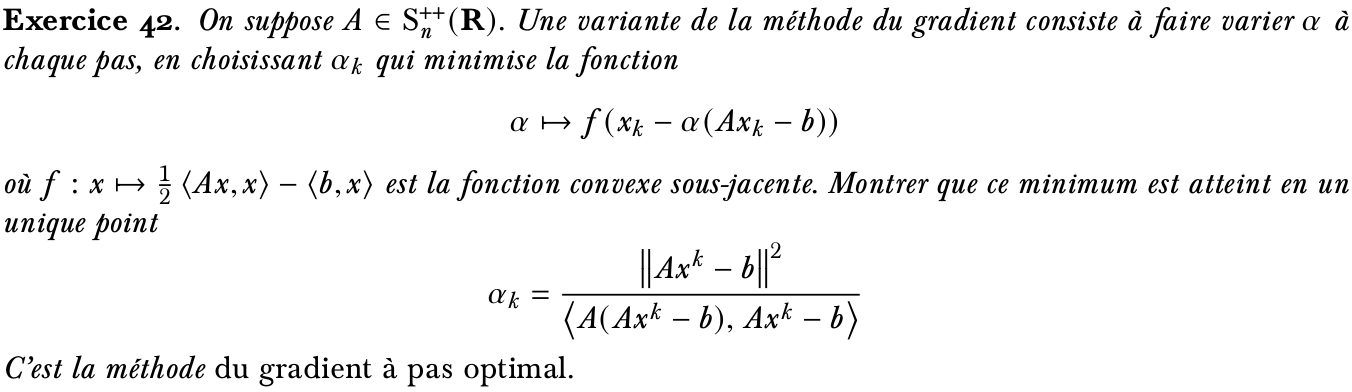
\includegraphics[width=\linewidth]{f/pasoptimal.png}
\vfill
\end{frame}


\begin{frame}
ITÉRATIONS DU GRADIENT\\
======================

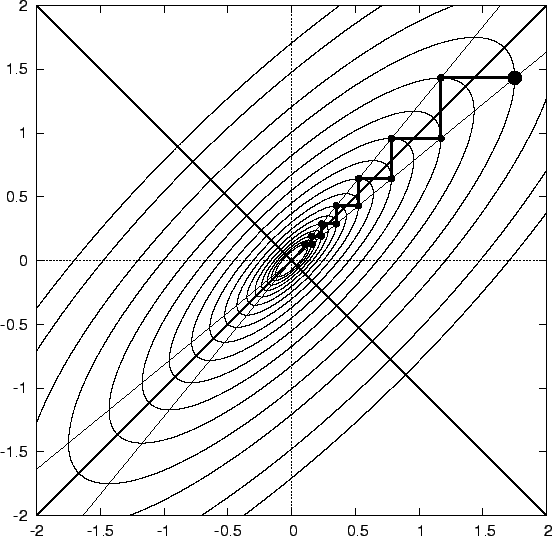
\includegraphics[width=0.53\linewidth]{f/iterationsgpo.png}%
\pause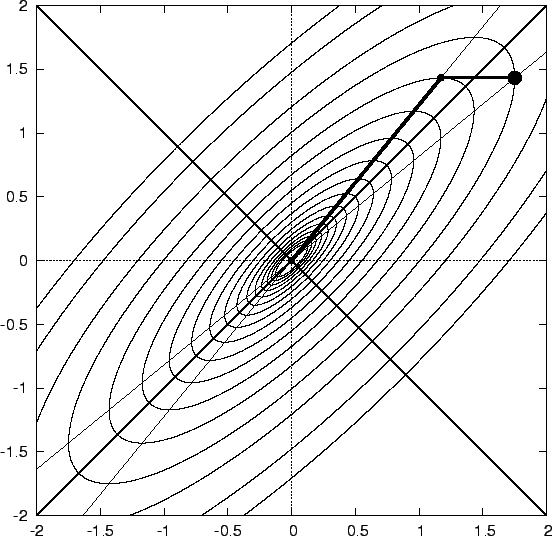
\includegraphics[width=0.53\linewidth]{f/iterationsgc.png}

gradient euclidien vs. gradient ``conjugué''

\end{frame}

% gradient conjugué
\begin{frame}
GRADIENT CONJUGUÉ 1/3\\
=====================

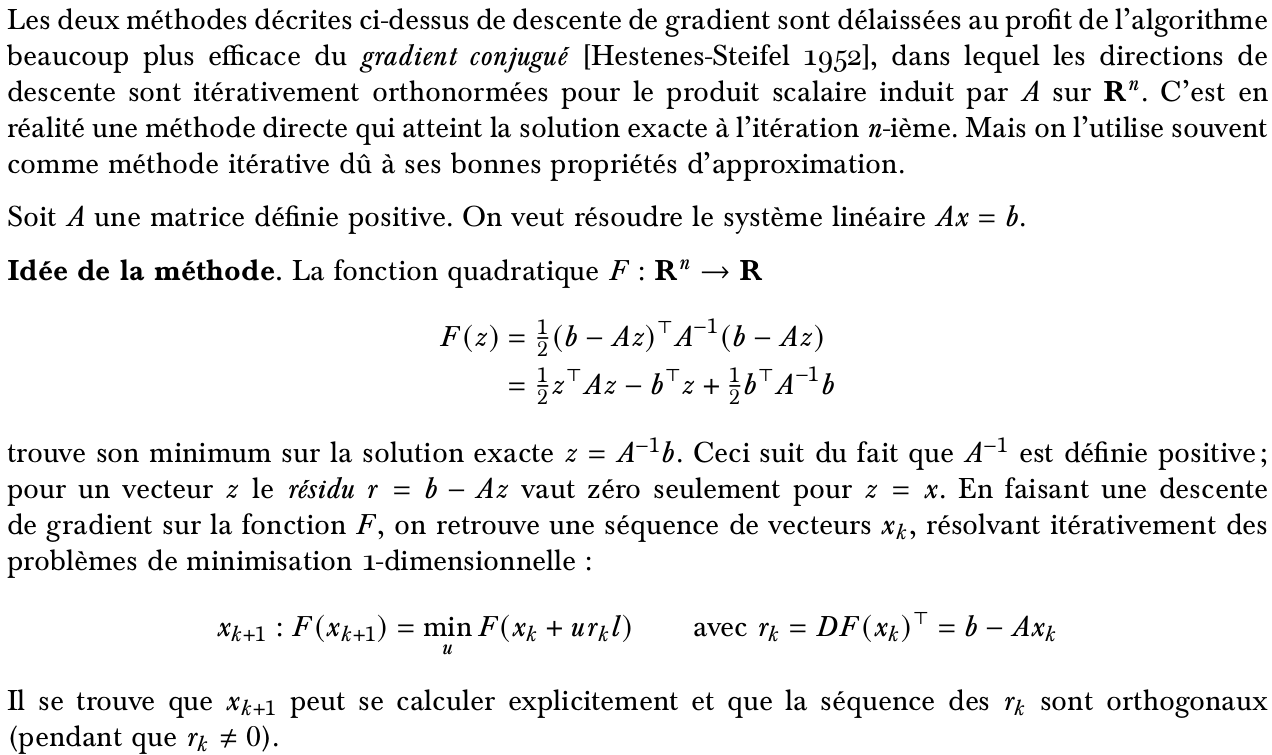
\includegraphics[width=\linewidth]{f/gradconj1.png}
\end{frame}

\begin{frame}
GRADIENT CONJUGUÉ 2/3\\
=====================

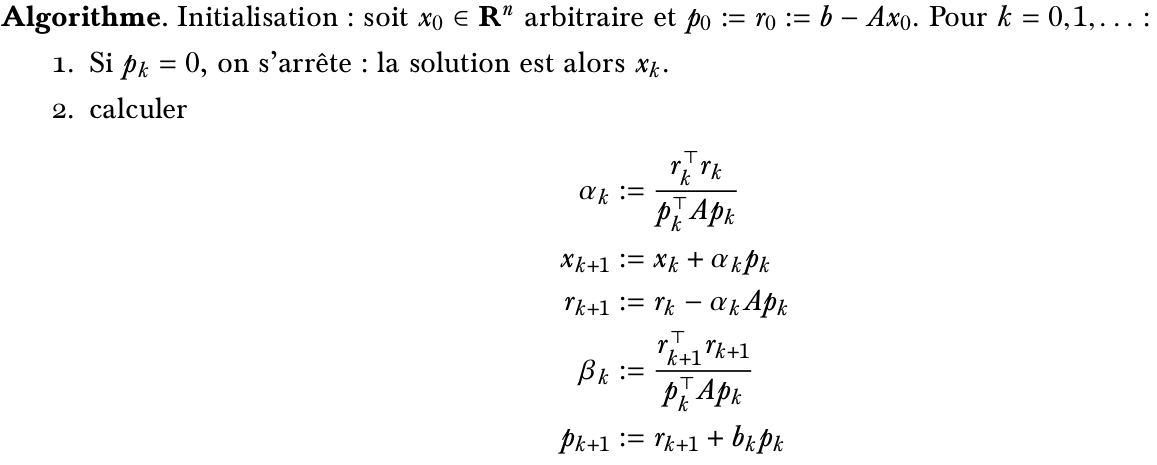
\includegraphics[width=\linewidth]{f/gradconj2.png}
\end{frame}

\begin{frame}
GRADIENT CONJUGUÉ 3/3\\
=====================

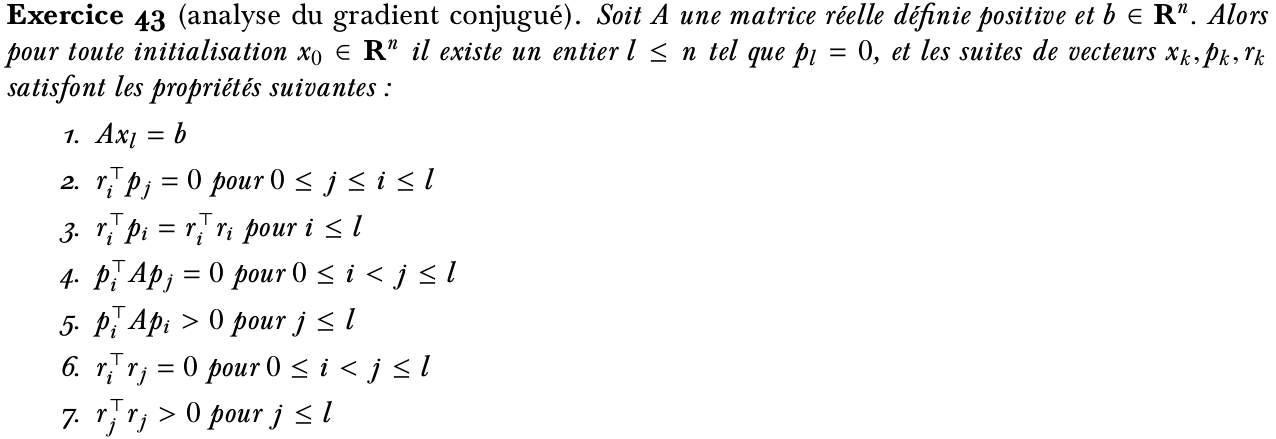
\includegraphics[width=\linewidth]{f/gradconj3.png}
\end{frame}

% modélisation: spectre du laplacien (avec plusieurs conditions de bord
% différentes) [EX]
\begin{frame}
MODÉLISATION: LE LAPLACIEN DISCRET 1D\\
=====================================

\vfill
voir {\color{red}\bf exercice L} en pièce jointe (lapdisc.pdf)
\vfill
\end{frame}



\begin{frame}
RÉSUMÉ\\
======

0. Interlude: résolution d'équations non-linéaires\\
$\ $0.1. Dichotomie\\
$\ $0.2. Méthode de Newton\\
$\ $0.3. Région de convergence, taux de convergence

1. Méthodes itératives pour éléments propres\\
$\ $1.1. Méthode de la puissance\\
$\ $1.2. Méthodes de la puissance inverse et guidée\\
$\ $1.3. Algorithme QR

2. Méthodes itératives pour systèmes linéaires\\
$\ $2.1. Cadre général\\
$\ $2.2. Jacobi, Gauss-Seidel, S.O.R.\\
$\ $2.3. Descente de gradient à pas fixe, à pas optimal\\
$\ $2.4. Gradients conjugués


\end{frame}


\begin{frame}
REPARTITION DES EXERCICES\\
=========================

%{\bf Tous:} Exercices 1, 2 (intersection de groupes) et 5.\\
%{\bf Groupe 1:} Exercice 3 (théorème spectral)\\
%{\bf Groupe 2:} Exercices 4 et 6 (éléments propres)\\
%{\bf Groupe 3:} Exercice 7 (théorème du min-max)\\
%{\bf Groupe 4:} Exercice 8 et 9 (disques de Gershgorin)\\
%{\bf Groupe 5:} Exercice 12 et 13 (décomposition polaire)\\
%{\bf Groupe 6:} Exercice 14, 15 et 17 (pseudo-inverse)\\
{\bf Groupe 1:} Exercices N, N' (Newton)\\
{\bf Groupe 2:} Exercice 36 (méthode de la puissance)\\
{\bf Groupe 3:} Exercice 37 (puissance inverse)\\
{\bf Groupe 4:} Exercice 40 (Gauss-Seidel)\\
{\bf Groupe 5:} Exercices 41, 42 (descente de gradient)\\
{\bf Groupe 6:} Exercice P (laplacien discret, système)\\
{\bf Groupe 7:} Exercice L (laplacien discret, spectre)\\


\vfill
Temps:\\
{\bf 90min} travail en groupe (6 groupes de 2,3 personnes)\\
{\bf 60min} mise en commun
(6 présentations de 10min par les ``scribes'' de chaque groupe)

\vfill
\color{red}
{\bf
Scribes: veuillez m'envoyer vos productions\\
(même incomplètes)}

\end{frame}

\end{document}


% vim:sw=2 ts=2 spell spelllang=fr:
